\chapter{Resultados}
\chaptermark{Resultados}
\label{chap:desarrollo}

\drop{E}{ste} capítulo constituye el núcleo del trabajo y presenta los
resultados del desarrollo de \dataqual en su dimensión real: qué se planificó
hacer, qué se hizo efectivamente y cómo se hizo, iteración por iteración.
Comienza con el análisis funcional del sistema (sus casos de uso) y se
estructura a continuación en seis sprints, cada uno con sus subsecciones de
planificación, trabajo realizado, evidencias técnicas (\emph{cómo se ha
hecho}) y retrospectiva.  Tras los sprints, varias secciones transversales
recogen los resultados globales del sistema (cuantitativos, calidad del
código, esfuerzo y cumplimiento de requisitos no funcionales) y la cobertura
alcanzada respecto al marco \ac{ISO}/\ac{IEC}~5259.

La estructura por sprints agrupa el desarrollo en \textbf{dominios
funcionales}: análisis y arquitectura (S1), núcleo del \emph{backend}
(S2), motor de métricas (S3), interfaz de usuario (S4), funcionalidades
avanzadas (S5) y consolidación (S6).  Como es habitual en un proceso
iterativo, las actividades de un dominio no se cerraron herméticamente al
finalizar el sprint correspondiente: algunos componentes (como el
\emph{watchdog} de evaluaciones, el versionado de datasets, el sistema
de \emph{Quality Gates} o ciertos elementos de internacionalización) se
iniciaron en un sprint y se refinaron o consolidaron en sprints
posteriores a medida que las dependencias quedaban disponibles.  Las tablas de \emph{story points} y horas reflejan, para
cada sprint, el trabajo principal del dominio correspondiente, mientras
que la narrativa describe cada componente en el sprint donde alcanzó su
versión funcional definitiva.


%% =========================================================================
\section{Análisis funcional}
\label{sec:requisitos-globales}
%% =========================================================================

El análisis funcional de \dataqual se expresa mediante sus \textbf{casos de
uso}, que describen las interacciones de los actores con el sistema.

El sistema soporta dos actores: \textbf{Usuario autenticado} (actor
principal, único rol con interfaz de usuario en esta versión, con acceso
a la gestión de proyectos, datasets, métricas, evaluaciones, Quality
Gates y exploración de datos) y \textbf{Sistema} (actor interno que
ejecuta las tareas asíncronas de evaluación y supervisa su estado).  Sobre
estos dos actores se definen \textbf{ocho casos de uso} que cubren la
totalidad del comportamiento funcional de \dataqual, sintetizados en el
diagrama de la Figura~\ref{fig:casos-uso}.  La especificación textual de
cada uno se recoge en el Anexo~\ref{anx:diagramas}.

\begin{figure}[htbp]
  \centering
  \begin{tikzpicture}[
      actor/.pic={
        \draw[thick] (0,0.6) circle [radius=0.13];
        \draw[thick] (0,0.47) -- (0,0);
        \draw[thick] (-0.22,0.3) -- (0.22,0.3);
        \draw[thick] (0,0) -- (-0.18,-0.32);
        \draw[thick] (0,0) -- (0.18,-0.32);
      },
      usecase/.style={ellipse, draw, thick, align=center,
                      font=\footnotesize,
                      minimum width=3.4cm, minimum height=0.7cm,
                      inner sep=1pt},
      uses/.style={-, thick},
    ]
    %% Casos de uso (columna central, dentro del límite del sistema)
    \node[usecase] (uc01) at (0, 3.6)  {UC-01 Gestionar proyectos};
    \node[usecase] (uc02) at (0, 2.7)  {UC-02 Gestionar datasets};
    \node[usecase] (uc03) at (0, 1.8)  {UC-03 Configurar métricas};
    \node[usecase] (uc04) at (0, 0.9)  {UC-04 Ejecutar evaluación};
    \node[usecase] (uc05) at (0, 0)    {UC-05 Gestionar Quality Gate};
    \node[usecase] (uc06) at (0,-0.9)  {UC-06 Explorar datos (\ac{EDA})};
    \node[usecase] (uc07) at (0,-2.1)  {UC-07 Ejecutar tarea asíncrona};
    \node[usecase] (uc08) at (0,-3.0)  {UC-08 Detectar evaluaciones atascadas};

    %% Límite del sistema
    \begin{pgfonlayer}{background}
      \node[draw, thick, rounded corners=3pt, inner sep=15pt,
            fit=(uc01)(uc08),
            label={[font=\small\bfseries]above:DataQual}] (sys) {};
    \end{pgfonlayer}

    %% Actores
    \pic at (-5.6, 1.35) {actor};
    \node[font=\small, align=center] at (-5.6, 0.55) {Usuario\\autenticado};

    \pic at (5.6,-2.55) {actor};
    \node[font=\small, align=center] at (5.6,-3.35) {Sistema\\(interno)};

    %% Asociaciones del Usuario con UC-01..UC-06
    \foreach \uc in {uc01,uc02,uc03,uc04,uc05,uc06}
      \draw[uses] (-5.25, 1.35) -- (\uc.west);

    %% Asociaciones del Sistema (interno) con UC-07, UC-08
    \draw[uses] (5.25,-2.55) -- (uc07.east);
    \draw[uses] (5.25,-2.55) -- (uc08.east);
  \end{tikzpicture}
  \caption{Diagrama \ac{UML} de casos de uso de \dataqual}
  \label{fig:casos-uso}
\end{figure}


%% =========================================================================
\section{Sprint 1: Análisis, arquitectura y setup inicial}
\label{sec:sprint1}
\textit{Período: agosto--septiembre 2025 \quad Duración: 8 semanas \quad SP: 13}
%% =========================================================================

\subsection{Trabajo realizado}

\textbf{Objetivo del sprint:} diseñar la arquitectura completa del sistema,
definir el modelo de datos inicial y poner en marcha el entorno de desarrollo
Docker con todos los servicios básicos operativos. Este sprint sentó las bases
para la autenticación de usuarios mediante tokens \ac{JWT}, el diseño del
diagrama entidad-relación (\ac{ERD}) y la posterior implementación de las
operaciones \ac{CRUD} sobre los recursos.

\begin{table}[htbp]
  \centering
  \small
  \caption{Sprint 1: Historias de usuario y estimación}
  \label{tab:sprint1-hu}
  \begin{tabularx}{\textwidth}{l X c c}
    \toprule
    \textbf{ID} & \textbf{Ítem} & \textbf{Est. (SP)} & \textbf{Real (h)} \\
    \midrule
    HU-01 & Registro e inicio de sesión básico & 3 & 10 \\
    HU-02 & JWT: access + refresh token & 2 & 8 \\
    T-01  & Setup Docker Compose (8 servicios) & 3 & 14 \\
    T-02  & Diseño del modelo de datos (\ac{ERD}) & 3 & 12 \\
    T-03  & Migraciones iniciales (Flask-Migrate) & 2 & 16 \\
    --    & Prueba de concepto: subida de dataset \ac{CSV} & 0 & --- \\
    \midrule
    \multicolumn{2}{l}{\textbf{Total}} & \textbf{13 SP} & \textbf{60 h} \\
    \bottomrule
  \end{tabularx}
\end{table}

\textbf{Dependencias y riesgos detectados:} la configuración de Docker Compose
con \emph{healthchecks} y dependencias entre servicios era desconocida al
inicio, constituyendo el principal riesgo (R-02 del plan de riesgos).

Se completaron los ítems del sprint con las siguientes observaciones:

\begin{itemize}
  \item El entorno Docker Compose quedó completamente operativo con los ocho
    servicios, \emph{healthchecks}, red interna y volúmenes persistentes.
  \item Se diseñó el modelo de datos inicial con campos JSONB para
    flexibilidad futura.  El esquema evolucionó en sprints posteriores hasta
    alcanzar las once tablas del sistema final.
  \item Se implementó el módulo de autenticación JWT completo con registro,
    login, refresco de token y revocación por \ac{JTI} (en memoria; los tokens
    revocados no persisten entre reinicios del servidor).
  \item Se realizó una prueba de concepto de subida de archivo \ac{CSV} al sistema:
    el endpoint básico de carga almacena el fichero en MinIO y registra los
    metadatos en la tabla \texttt{datasets}.  La implementación completa del
    módulo de ingesta se completó en el Sprint~2.
  \item \textbf{Cambio respecto a lo planificado}: la configuración de
    \emph{healthchecks} en Docker Compose requirió más tiempo del estimado
    (+4h) debido a los tiempos de arranque de PostgreSQL y MinIO.
\end{itemize}

\subsection{Cómo se ha hecho}

\subsubsection{Arquitectura general del sistema}
\label{sec:arquitectura}

\dataqual sigue una arquitectura de \textbf{servicios orquestados} mediante
Docker Compose~\citep{docker}.  Los ocho servicios que componen la plataforma
se comunican a través de una red interna (\texttt{app-network}, \emph{driver}
\emph{bridge}) y exponen al anfitrión únicamente los puertos necesarios.

La Figura~\ref{fig:arquitectura-componentes} ofrece una visión de conjunto:
distingue la \textbf{aplicación} (software) de la \textbf{infraestructura}
y muestra las relaciones entre componentes con su protocolo de comunicación.

\begin{figure}[htbp]
  \centering
  
\includegraphics[width=\textwidth]{img/arquitectura-componentes.png}
  \caption{Arquitectura de componentes de \dataqual: separación entre
    aplicación (software) e infraestructura, con las relaciones y
    protocolos de comunicación entre componentes}
  \label{fig:arquitectura-componentes}
\end{figure}

El Cuadro~\ref{tab:servicios} recoge los ocho servicios, sus puertos y su
propósito.

\begin{table}[htbp]
  \centering
  \caption{Servicios Docker de \dataqual}
  \label{tab:servicios}
  \begin{tabularx}{\textwidth}{l c X}
    \toprule
    \textbf{Servicio} & \textbf{Puerto} & \textbf{Propósito} \\
    \midrule
    \texttt{frontend}      & 3000 & Interfaz de usuario (Next.js + React) \\
    \texttt{backend}       & 5000 & \ac{API} \ac{REST} (Flask + Gunicorn) \\
    \texttt{postgres}      & 5432 & Base de datos relacional (PostgreSQL~14) \\
    \texttt{minio}         & 9000/9001 & Almacenamiento de objetos S3 \\
    \texttt{redis}         & 6379 & \emph{Broker} de mensajes y caché \\
    \texttt{celery-worker} & --- & Ejecución asíncrona de evaluaciones \\
    \texttt{celery-beat}   & --- & Programación de tareas periódicas \\
    \texttt{flower}        & 5555 & Monitorización de Celery \\
    \bottomrule
  \end{tabularx}
\end{table}

El flujo de comunicación entre servicios se organiza de la siguiente manera:
el \emph{frontend} (Next.js) realiza peticiones HTTP/JSON al \emph{backend}
(Flask); éste lee y escribe en PostgreSQL (datos relacionales), MinIO
(archivos binarios) y Redis (caché y \emph{broker}); cuando el usuario lanza
una evaluación, el \emph{backend} encola una tarea en Redis que es consumida
por el \emph{Celery worker}.

El Cuadro~\ref{tab:comunicacion} resume los protocolos de comunicación.

\begin{table}[htbp]
  \centering
  \caption{Protocolos de comunicación entre componentes}
  \label{tab:comunicacion}
  \begin{tabularx}{\textwidth}{l l l X}
    \toprule
    \textbf{Origen} & \textbf{Destino} & \textbf{Protocolo} &
      \textbf{Mecanismo} \\
    \midrule
    Frontend & Backend    & HTTP/JSON & Next.js (\emph{rewrite} \texttt{/api/*}),
      cliente Axios \\
    Backend  & PostgreSQL & TCP       & SQLAlchemy \ac{ORM} (\emph{pool} de
      10 conexiones) \\
    Backend  & MinIO      & HTTP/S3   & Cliente MinIO para Python \\
    Backend  & Redis      & TCP       & Celery \emph{broker} + Flask-Limiter \\
    Worker   & Redis      & TCP       & Consumo de tareas del \emph{broker} \\
    Worker   & PostgreSQL & TCP       & Actualización de progreso y resultados \\
    Worker   & MinIO      & HTTP/S3   & Descarga de conjuntos de datos \\
    \bottomrule
  \end{tabularx}
\end{table}

Todos los servicios poseen una política de reinicio \texttt{unless-stopped}
y los servicios de infraestructura incluyen \emph{healthchecks} que verifican
su disponibilidad antes de que arranquen los servicios dependientes.

\subsubsection{Modelo de datos}
\label{sec:modelo-datos}

PostgreSQL~14~\citep{postgresql} almacena todos los datos relacionales y
metadatos del sistema.  El esquema final comprende \textbf{once tablas}
organizadas en tres grupos: identidad y proyectos (\texttt{users},
\texttt{projects}, \texttt{datasets}, \texttt{metrics},
\texttt{metric\_templates}), subsistema de análisis incremental
(\texttt{analysis\_runs}, \texttt{data\_quality\_issues},
\texttt{quality\_gates}, \texttt{validation\_patterns}) y modelo original
mantenido por retrocompatibilidad (\texttt{evaluations},
\texttt{issues}).  En este sprint se crearon las siete iniciales; las
cuatro del subsistema de análisis incremental se incorporaron en el Sprint~5.  El
diseño hace un uso extensivo de campos \textbf{JSONB} para almacenar
estructuras semiestructuradas que varían según la métrica o
configuración: \texttt{projects.metrics\_config},
\texttt{datasets.schema}, \texttt{datasets.sensitive\_columns},
\texttt{quality\_gates.thresholds} y \texttt{analysis\_runs.results}.
El versionado de \emph{datasets} se implementa mediante el par
\texttt{parent\_dataset\_id} + \texttt{is\_latest}.  El esquema
completo (tablas, columnas, tipos y relaciones de clave foránea) se
representa en la Figura~\ref{fig:er-diagram}: las columnas marcadas con
\texttt{\{\}} corresponden a campos JSONB y la tabla
\texttt{alembic\_version} es interna de Flask-Migrate (control de
migraciones), ajena al dominio.

\begin{figure}[htbp]
  \centering
  
\includegraphics[width=\textwidth,height=0.82\textheight,keepaspectratio]{img/er-diagram.png}
  \caption[Esquema relacional de la base de datos \texttt{dataquality}]{Esquema
    relacional de la base de datos \texttt{dataquality}: tablas, columnas, tipos
    y relaciones de clave foránea.  Iconos de tipo (DBeaver):
    \texttt{123}~numérico, \texttt{A-Z}~texto, reloj~fecha/hora,
    casilla~booleano y \texttt{\{\}}~JSONB.}
  \label{fig:er-diagram}
\end{figure}

\subsection{Retrospectiva}

\begin{table}[htbp]
  \centering
  \small
  \caption{Sprint 1: Retrospectiva}
  \label{tab:sprint1-retro}
  \begin{tabularx}{\textwidth}{l X}
    \toprule
    \textbf{Aspecto} & \textbf{Detalle} \\
    \midrule
    Conseguido & Entorno de desarrollo operativo, arquitectura documentada,
      autenticación JWT y prueba de concepto de subida de dataset \ac{CSV}. \\
    Pendiente & Ningún ítem quedó sin completar; las migraciones del esquema
      requerirán iteraciones conforme evolucione el modelo. \\
    Qué fue bien & Definir el modelo de datos completo desde el inicio evitó
      migraciones disruptivas posteriores. \\
    Qué fue mal & La configuración de Docker Compose con \emph{healthchecks}
      resultó más compleja de lo previsto (+4\,h), sobre todo la secuencia de
      arranque entre servicios. \\
    Lección aprendida & Reservar tiempo explícito para infraestructura, que
      tiende a subestimarse. \\
    Acción de mejora & Añadir un 20\,\% de margen en las estimaciones de tareas
      de infraestructura. \\
    \bottomrule
  \end{tabularx}
\end{table}


%% =========================================================================
\section{Sprint 2: \emph{Backend} principal, datasets y \acs{API} \acs{REST}}
\label{sec:sprint2}
\textit{Período: enero 2026 \quad Duración: 4 semanas \quad SP: 18}
%% =========================================================================

\subsection{Trabajo realizado}

\textbf{Objetivo del sprint:} implementar el módulo de ingesta y
almacenamiento de datasets, la arquitectura completa del \emph{backend} en
capas, la \ac{API} \ac{REST} y la gestión de proyectos.

\begin{table}[htbp]
  \centering
  \small
  \caption{Sprint 2: Historias de usuario y estimación}
  \label{tab:sprint2-hu}
  \begin{tabularx}{\textwidth}{l X c c}
    \toprule
    \textbf{ID} & \textbf{Ítem} & \textbf{Est. (SP)} & \textbf{Real (h)} \\
    \midrule
    HU-03 & \ac{CRUD} de proyectos + configuración de métricas & 3 & 12 \\
    HU-05 & Carga y parseo robusto de archivos \ac{CSV} & 5 & 22 \\
    HU-06 & Versionado de datasets (parent-child, is\_latest) & 3 & 10 \\
    T-04  & Arquitectura del backend en capas (blueprints, servicios) & 4 & 18 \\
    T-05  & Especificación y pruebas manuales de la API \ac{REST} & 3 & 23 \\
    \midrule
    \multicolumn{2}{l}{\textbf{Total}} & \textbf{18 SP} & \textbf{85 h} \\
    \bottomrule
  \end{tabularx}
\end{table}

\textbf{Dependencias}: requiere Sprint~1 completado (base de datos y
autenticación operativos).  \textbf{Riesgo principal}: la diversidad de
formatos de archivo y codificaciones de \ac{CSV} puede generar una estrategia de
\emph{fallback} más compleja de lo previsto (R-03).

\begin{itemize}
  \item Implementada la arquitectura del \emph{backend} en capas: \emph{blueprints}
    Flask, capa de servicio y \emph{middleware}.
  \item Desarrollado el módulo de ingesta \ac{CSV} con estrategia de
    \emph{fallback} múltiple: cuatro codificaciones (UTF-8, UTF-8 con
    \ac{BOM}, CP1252, Latin-1), seis estrategias de separador (los cuatro
    candidatos explícitos más el delimitador inferido por
    \texttt{csv.Sniffer} y la autodetección de Pandas) y los dos motores
    de \emph{parsing} de Pandas.
  \item Implementado el versionado de datasets con relaciones parent-child.
  \item Completados los seis módulos funcionales de la \ac{API} \ac{REST}
    con formato de respuesta estandarizado y paginación.  Durante la
    implementación se añadieron tres \emph{blueprints} adicionales por
    convención \ac{REST}: \texttt{project\_metrics} y \texttt{project\_datasets}
    (sub-rutas anidadas \texttt{/projects/<id>/…}) y \texttt{dashboard}
    (agregación de solo lectura), elevando el total a nueve \emph{blueprints}
    Flask registrados, que en el Sprint~5 ascenderían a diez con la
    incorporación de \texttt{patterns}.
  \item \textbf{Cambio respecto a lo planificado}: el parseo robusto de \ac{CSV}
    requirió una semana adicional por la casuística de ficheros con \ac{BOM},
    delimitadores inusuales y codificaciones mixtas.
\end{itemize}

\subsection{Cómo se ha hecho}

\subsubsection{Arquitectura del \emph{backend}}
\label{sec:arq-backend}

El \emph{backend} sigue una \textbf{arquitectura en capas} con separación
clara de responsabilidades.

La Figura~\ref{fig:diagrama-paquetes} sitúa el \emph{backend} en el conjunto
del sistema y muestra su organización en paquetes y las dependencias entre
capas (\texttt{api}~$\to$~\texttt{services}~$\to$~\texttt{metrics}/\texttt{models}).

\begin{figure}[htbp]
  \centering
  
\includegraphics[width=0.95\textwidth,keepaspectratio]{img/diagrama_paquetes.png}
  \caption{Diagrama de paquetes del sistema (Frontend y Backend)}
  \label{fig:diagrama-paquetes}
\end{figure}

La aplicación Flask se crea mediante el \textbf{patrón factoría}
(\texttt{create\_app()} en \texttt{app.py})~\citep{design_patterns}, que
inicializa las extensiones, registra los \emph{blueprints} y configura el
\emph{middleware}.  La \ac{API} se monta bajo el prefijo \texttt{/api}
y queda organizada en este sprint en \textbf{seis módulos funcionales}
(\texttt{auth}, \texttt{projects}, \texttt{datasets}, \texttt{metrics},
\texttt{evaluations}, \texttt{admin}) más tres \emph{blueprints} de
organización técnica derivados de la convención \ac{REST} de rutas anidadas
(\texttt{project\_metrics}, \texttt{project\_datasets},
\texttt{dashboard}).  En el Sprint~5 se incorporará un séptimo módulo
funcional (\texttt{patterns}), llegando al total final de diez
\emph{blueprints}.  La especificación completa
de rutas, parámetros y formatos de respuesta se encuentra en el
Anexo~\ref{anx:api}.

A modo de ilustración, el Listado~\ref{lst:api-ejemplo} muestra la creación
de un proyecto (\texttt{POST /api/projects/}) y su respuesta en el formato
estandarizado \texttt{\{success, data, message\}} común a toda la \ac{API}.

\begin{listing}[caption={Petición y respuesta de la API REST: creación de un proyecto},label={lst:api-ejemplo}]
POST /api/projects/
Authorization: Bearer <token>
Content-Type: application/json

{ "name": "Ventas Q1", "description": "Ventas del primer trimestre" }

==> 201 Created
{
  "success": true,
  "data": {
    "id": 7,
    "name": "Ventas Q1",
    "description": "Ventas del primer trimestre",
    "owner_id": 3,
    "metrics_config": [
      { "id": "completeness", "parameters": {} },
      { "id": "uniqueness",   "parameters": {} },
      { "id": "outliers", "parameters": { "method": "iqr", "factor": 1.5 } }
    ],
    "created_at": "2026-01-15T10:32:00",
    "updated_at": "2026-01-15T10:32:00",
    "dataset_count": 0
  },
  "message": "Proyecto creado correctamente"
}
\end{listing}

La lógica de negocio se encapsula en servicios independientes.  En este
sprint se establecieron los dos servicios fundamentales:
\texttt{DatasetService} (parseo y extracción de esquema) y
\texttt{MinioService} (abstracción sobre S3).  En sprints posteriores se
añadirán \texttt{EvaluationService} (S3, orquestación del flujo de
evaluación), \texttt{HybridEvaluationService} (S5, \emph{fallback}
síncrono) y \texttt{ExportService} (S5, generación de informes).

El \emph{backend} incorpora capas de \emph{middleware}: generación de
\texttt{X-Request-ID}, gestión centralizada de errores HTTP y monitor de
rendimiento por \emph{endpoint} (detecta peticiones lentas >500~ms),
establecidos en este sprint.  El \emph{Evaluation Watchdog} (hilo
\emph{daemon} que detecta evaluaciones atascadas) se incorporó en el
Sprint~3, una vez que las evaluaciones fueron operativas.

El sistema mantiene una \textbf{arquitectura dual de modelos} como resultado
de su evolución incremental.  El modelo original (\texttt{Evaluation} +
\texttt{Issue}), implementado en el Sprint~2, ofrecía una estructura sencilla
adecuada para la primera versión del proyecto.  Al diseñar en el Sprint~5 el sistema de
\emph{fingerprinting} y los \emph{Quality Gates}, resultó necesario un modelo
semánticamente más rico: el \textbf{subsistema de análisis incremental}
(\texttt{AnalysisRun} + \texttt{DataQualityIssue} + \texttt{QualityGate}),
que soporta comparación con línea base, contadores de \emph{issues}
nuevos/recurrentes/corregidos y configuración de umbrales por proyecto.
Ambos modelos coexisten para preservar la retrocompatibilidad con los
\emph{endpoints} implementados en sprints anteriores; la unificación
completa en un único modelo queda documentada como mejora futura en la
sección~\ref{sec:trabajo-futuro}.

\subsubsection{Módulo de ingesta y almacenamiento}
\label{sec:impl-ingesta}

Los usuarios pueden cargar archivos en formato \ac{CSV} con un límite de
tamaño configurable (por defecto, 100\,MB).  Tras superar la validación,
el fichero se persiste en MinIO como objeto binario y sus metadatos
(esquema inferido, tamaño, versión y proyecto al que pertenece) se
registran en PostgreSQL mediante el modelo \texttt{Dataset}.

El servicio \texttt{DatasetService} implementa una estrategia de lectura
robusta de \ac{CSV} estructurada en tres fases:

\begin{enumerate}
  \item \textbf{Validación del formato real:} se inspeccionan los
    primeros bytes del fichero para detectar archivos incorrectamente
    etiquetados como \ac{CSV}.  Los ficheros Excel (XLSX) se rechazan con
    un mensaje claro al usuario, mientras que los archivos comprimidos
    con \emph{gzip} se descomprimen de forma transparente antes de
    continuar.

  \item \textbf{Detección del delimitador:} se aplica
    \texttt{csv.Sniffer} sobre los primeros 8\,192 bytes del contenido,
    evaluando los candidatos coma, punto y coma, tabulador y
    \emph{pipe}.

  \item \textbf{Matriz de \emph{fallback}:} si la detección del
    delimitador no es concluyente o la lectura no produce un
    \emph{DataFrame} válido, se ensayan exhaustivamente combinaciones de
    cuatro codificaciones (UTF-8, UTF-8 con \ac{BOM}, CP1252, Latin-1), seis
    estrategias de separador (el detectado, la inferencia automática de
    Pandas y los cuatro candidatos explícitos) y los dos motores de
    \emph{parsing} de Pandas (Python y C).  Se retorna el primer intento
    que produzca columnas válidas.
\end{enumerate}

Al cargar un conjunto de datos, el sistema extrae automáticamente el
nombre y tipo de cada columna, estadísticas descriptivas y histogramas
para columnas numéricas.  El versionado opera mediante un campo
\texttt{parent\_dataset\_id} opcional y un indicador \texttt{is\_latest}:
las cargas sucesivas dentro de un mismo proyecto generan versiones
encadenadas que conservan el historial completo.  La Figura~\ref{fig:dataset-lineage} presenta el árbol visual interactivo
(\emph{Visual version tree}) de un \emph{dataset}, con nodos coloreados según
el estado de \emph{Quality Gate} y el diferencial de puntuación entre
versiones padre-hijo.  La lista cronológica de versiones
(Figura~\ref{fig:dataset-versions-list}) y la comparación entre dos versiones,
con su desglose de \emph{issues} resueltos, nuevos y persistentes
(Figura~\ref{fig:version-comparison}), se recogen en el manual de usuario
(Anexo~\ref{anx:manual}).

\begin{figure}[htbp]
  \centering
  
\includegraphics[width=0.8\textwidth]{img/dataset-lineage.png}
  \caption{Canvas de árbol de versiones (\emph{Visual version tree}):
    grafo interactivo con nodos coloreados por estado de \emph{Quality Gate}
    y diferencial de puntuación entre versiones padre-hijo}
  \label{fig:dataset-lineage}
\end{figure}

\subsubsection{\acs{API} \acs{REST}ful}
\label{sec:impl-api}

La \ac{API} \ac{REST}ful presenta las siguientes características transversales:
autenticación \ac{JWT} en todos los \emph{endpoints} protegidos, formato de
respuesta estandarizado \texttt{\{success, data, message\}}, paginación con
parámetros \texttt{page}/\texttt{per\_page}, y validación mediante esquemas
Marshmallow.  La especificación completa de \emph{endpoints} se recoge en el
Anexo~A.

\subsection{Retrospectiva}

\begin{table}[htbp]
  \centering
  \small
  \caption{Sprint 2: Retrospectiva}
  \label{tab:sprint2-retro}
  \begin{tabularx}{\textwidth}{l X}
    \toprule
    \textbf{Aspecto} & \textbf{Detalle} \\
    \midrule
    Conseguido & \emph{Backend} funcional con todos los módulos principales,
      \ac{API} \ac{REST} operativa y datasets versionados. \\
    Pendiente & Motor de métricas (HU-07, HU-09, HU-10) y \emph{frontend}
      completo (HU-04, HU-13, HU-14) programados para S3 y S4. \\
    Qué fue bien & La separación en capas (\emph{blueprints} + servicios)
      facilita las pruebas y la extensión futura. \\
    Qué fue mal & El parseo robusto de \ac{CSV} resultó mucho más complejo de
      lo esperado; la diversidad de codificaciones y delimitadores reales
      obligó a extender el sprint una semana. \\
    Lección aprendida & Los datos reales son más irregulares que los formatos
      estándar; conviene aplicar estrategias defensivas desde el inicio. \\
    Acción de mejora & Crear una batería de datasets de prueba con casos
      extremos (\ac{BOM}, delimitadores inusuales, caracteres especiales) para
      validar el parseo. \\
    \bottomrule
  \end{tabularx}
\end{table}


%% =========================================================================
\section{Sprint 3: Motor de métricas de calidad}
\label{sec:sprint3}
\textit{Período: febrero 2026 \quad Duración: 4 semanas \quad SP: 16}
%% =========================================================================

\subsection{Trabajo realizado}

\textbf{Objetivo del sprint:} diseñar e implementar el motor de métricas con
arquitectura de \emph{plugins} y las tres primeras métricas de calidad,
alineadas con \ac{ISO}/\ac{IEC}~25012 e \ac{ISO}/\ac{IEC}~5259.

\begin{table}[htbp]
  \centering
  \small
  \caption{Sprint 3: Historias de usuario y estimación}
  \label{tab:sprint3-hu}
  \begin{tabularx}{\textwidth}{l X c c}
    \toprule
    \textbf{ID} & \textbf{Ítem} & \textbf{Est. (SP)} & \textbf{Real (h)} \\
    \midrule
    HU-07 & Configuración de métricas con parámetros y pesos & 5 & 20 \\
    HU-08 & Plantillas de métricas del sistema & 3 & 10 \\
    HU-09 & Lanzamiento de evaluación (tarea Celery, parte 1 de 2) & 5 & 22 \\
    HU-10 & Listado de issues con severidad & 3 & 18 \\
    \midrule
    \multicolumn{2}{l}{\textbf{Total}} & \textbf{16 SP} & \textbf{70 h} \\
    \bottomrule
  \end{tabularx}
\end{table}

\textbf{Dependencias}: requiere Sprint~2 completado (API \ac{REST} y datasets
operativos).

\begin{itemize}
  \item Diseñada e implementada la arquitectura de \emph{plugins} del motor
    de métricas (\texttt{BaseMetric}, \texttt{MetricResult},
    \texttt{METRIC\_REGISTRY}).
  \item Implementadas las tres primeras métricas evaluables del catálogo:
    completitud (\texttt{completeness}), unicidad (\texttt{uniqueness}) y
    consistencia lógica (\texttt{logical\_consistency}).  Paralelamente se
    implementó la clase \texttt{OutliersMetric}, usada solo en el módulo de
    perfilado de datos y excluida del \emph{Quality Score} por diseño.
  \item Implementada la fórmula del \emph{Quality Score} con penalización por
    issues.
  \item Integrada la ejecución asíncrona con Celery.
\end{itemize}

\subsection{Cómo se ha hecho}

\subsubsection{Arquitectura del motor de métricas}
\label{sec:motor-metricas}

El motor de métricas constituye el núcleo funcional de \dataqual.  Su diseño
se basa en una arquitectura de \emph{plugins} que permite añadir nuevas
métricas sin modificar el código existente.

La Figura~\ref{fig:diagrama-clases} representa la jerarquía de clases del motor
de métricas y los servicios asociados.

\begin{landscape}
\begin{figure}
  \centering
  
\includegraphics[width=\linewidth,keepaspectratio]{img/diagrama_clases.png}
  \caption{Diagrama de clases del motor de métricas y los servicios asociados}
  \label{fig:diagrama-clases}
\end{figure}
\end{landscape}

La arquitectura se compone de tres elementos:

\begin{definitionlist}
  \item[\texttt{BaseMetric}]  Clase base abstracta que define la interfaz
    que toda métrica debe implementar: el método \texttt{evaluate()}, que
    recibe un \emph{DataFrame} de Pandas, los parámetros configurados y
    devuelve un objeto \texttt{MetricResult}.  La clase base proporciona
    además métodos auxiliares para el cálculo de severidad dinámica, la
    generación de histogramas, la inferencia de tipos de columna y el
    enmascaramiento de valores sensibles.

  \item[\texttt{MetricResult}]  Estructura de datos (\emph{dataclass}) que
    encapsula el resultado de una evaluación: identificador de la métrica,
    puntuación (0,0--1,0), resultados detallados y lista de \emph{issues}
    detectados.

  \item[\texttt{METRIC\_REGISTRY}]  Diccionario que asocia cada
    identificador de métrica a su clase implementadora, permitiendo la
    instanciación dinámica por nombre.
\end{definitionlist}

Para añadir una nueva métrica basta con: (1)~crear una clase heredera de
\texttt{BaseMetric} que implemente \texttt{evaluate()}; (2)~registrarla en
\texttt{METRIC\_REGISTRY}; (3)~añadir la función de \emph{fingerprint};
y (4)~documentarla en el Anexo~B.

\subsubsection{Catálogo de métricas implementadas}

El motor incorpora progresivamente, a lo largo de los sprints S3, S4 y S5,
\textbf{siete métricas evaluables} que contribuyen al \emph{Quality Score}:
completitud (\texttt{completeness}), unicidad (\texttt{uniqueness}),
exactitud sintáctica (\texttt{syntactic\_accuracy}), consistencia lógica
(\texttt{logical\_consistency}), actualidad (\texttt{currentness}),
equilibrio de clases (\texttt{class\_balance}) y diversidad
(\texttt{diversity}).  Las fórmulas se alinean con \ac{ISO}/\ac{IEC}~25024
para las cuatro dimensiones inherentes y con \ac{ISO}/\ac{IEC}~5259-2 para
unicidad, equilibrio y diversidad.  Adicionalmente, la clase
\texttt{OutliersMetric} detecta valores atípicos mediante \ac{IQR}; por
recomendación de \ac{ISO}/\ac{IEC}~5259, no figura en
\texttt{METRIC\_REGISTRY} ni contribuye al \emph{Quality Score}, sino
que se utiliza únicamente como herramienta de diagnóstico en el módulo
\acs{EDA}.

La especificación detallada de cada métrica (fórmula, parámetros,
umbrales por defecto y generación de \emph{issues}) se recoge en el
Anexo~\ref{anx:metricas}.

\subsubsection{Fórmula del \emph{Quality Score}}

La puntuación global de calidad ($Q \in [0{,}1]$) se calcula mediante un
modelo de \textbf{penalización por \emph{issues} con corrección
dimensional}.  Cada métrica produce una puntuación individual (ratio de
celdas válidas) que se expone en la interfaz como información de diagnóstico,
pero \textbf{no alimenta directamente} la nota final: una proporción pequeña
de errores graves puede hacer un conjunto de datos inutilizable aunque la
ratio global sea elevada.  El cálculo sigue tres pasos:

\begin{enumerate}
  \item \textbf{Penalización bruta por severidad:}  cada \emph{issue}
    detectado contribuye con un peso fijo según su nivel de severidad:
    \[
      p_{\mathrm{raw}} =
        0{,}12\cdot n_{\mathrm{crit}}
      + 0{,}05\cdot n_{\mathrm{high}}
      + 0{,}01\cdot n_{\mathrm{med}}
      + 0{,}003\cdot n_{\mathrm{low}}
    \]

  \item \textbf{Corrección dimensional:}  los conjuntos de datos con más
    columnas generan naturalmente más \emph{issues}.  Un factor de escala
    basado en la raíz cuadrada del número de columnas normaliza la
    penalización para que la misma \emph{densidad} de errores produzca la
    misma nota con independencia de la dimensionalidad del dataset:
    \[
      \sigma = \sqrt{\frac{\max(10,\; c)}{10}}
    \]
    donde $c$ es el número de columnas del conjunto de datos y $10$ es el
    número de referencia (dataset de anchura estándar).

  \item \textbf{Puntuación final:}
    \[
      Q = \max\!\Bigl(0,\;1 - \min\!\bigl(0{,}97,\; p_{\mathrm{raw}} / \sigma\bigr)\Bigr)
    \]
    La cota $0{,}97$ sobre la penalización normalizada garantiza que ningún
    dataset obtiene $Q=0$ por un único \emph{issue} crítico aislado,
    preservando la diferenciación entre conjuntos de datos muy deficientes.
\end{enumerate}

El diálogo de configuración detallada de una métrica (ajuste de umbrales con
controles deslizantes, selección de columnas objetivo y previsualización del
equivalente \acs{JSON} en tiempo real) se ilustra en la
Figura~\ref{fig:metric-config-detail} del manual de usuario
(Anexo~\ref{anx:manual}).

\subsection{Retrospectiva}

\begin{table}[htbp]
  \centering
  \small
  \caption{Sprint 3: Retrospectiva}
  \label{tab:sprint3-retro}
  \begin{tabularx}{\textwidth}{l X}
    \toprule
    \textbf{Aspecto} & \textbf{Detalle} \\
    \midrule
    Conseguido & Motor de métricas operativo con las tres primeras métricas
      (completitud, unicidad y consistencia lógica), \texttt{OutliersMetric}
      para perfilado, \emph{Quality Score} con corrección dimensional y
      arquitectura de \emph{plugins} extensible. \\
    Pendiente & \emph{Frontend} completo (HU-04, HU-13, HU-14) en S4 y
      funcionalidades diferenciadoras (HU-11, HU-12) en S5. \\
    Qué fue bien & La arquitectura de \emph{plugins} con
      \texttt{METRIC\_REGISTRY} demostró su valor: añadir cada métrica requirió
      modificar solo su fichero de implementación. \\
    Qué fue mal & La métrica de consistencia lógica presentó dificultades con
      la validación de seguridad de las expresiones \texttt{query()}; varias
      iteraciones para equilibrar flexibilidad y prevención de inyección. \\
    Lección aprendida & La seguridad de las métricas que ejecutan expresiones
      de usuario debe diseñarse desde el principio, no como parche posterior. \\
    Acción de mejora & Documentar la interfaz de cada métrica (\emph{inputs},
      \emph{outputs}, parámetros) antes de S4, para facilitar la integración
      con el \emph{frontend}. \\
    \bottomrule
  \end{tabularx}
\end{table}


%% =========================================================================
\section{Sprint 4: \emph{Frontend} e interfaz de usuario}
\label{sec:sprint4}
\textit{Período: marzo 2026 \quad Duración: 4 semanas \quad SP: 14}
%% =========================================================================

\subsection{Trabajo realizado}

\textbf{Objetivo del sprint:} desarrollar la interfaz de usuario completa con
Next.js y React, incluyendo el cuadro de mando, las páginas de gestión de
proyectos y datasets, los resultados de evaluación y el perfilado exploratorio
de datos (\ac{EDA}).

\begin{table}[htbp]
  \centering
  \small
  \caption{Sprint 4: Historias de usuario y estimación}
  \label{tab:sprint4-hu}
  \begin{tabularx}{\textwidth}{l X c c}
    \toprule
    \textbf{ID} & \textbf{Ítem} & \textbf{Est. (SP)} & \textbf{Real (h)} \\
    \midrule
    HU-04 & Cuadro de mando principal con resumen & 5 & 20 \\
    HU-09 & Progreso de evaluación en tiempo real (polling, parte 2 de 2) & 3 & 14 \\
    HU-13 & \ac{EDA}: histogramas, boxplots, correlaciones & 5 & 24 \\
    HU-14 & Marcado de columnas \ac{PII} en la \ac{UI} & 1 & 7 \\
    \midrule
    \multicolumn{2}{l}{\textbf{Total}} & \textbf{14 SP} & \textbf{65 h} \\
    \bottomrule
  \end{tabularx}
\end{table}

\textbf{Dependencias}: requiere Sprint~3 completado (motor de métricas
operativo y \ac{API} de evaluaciones funcional para poder visualizar
resultados desde el \emph{frontend}).

\begin{itemize}
  \item Incorporadas tres métricas evaluables adicionales al catálogo:
    exactitud sintáctica (\texttt{syntactic\_accuracy}), equilibrio de clases
    (\texttt{class\_balance}) y actualidad (\texttt{currentness}), completando
    seis de las siete métricas evaluables del sistema.
  \item Desarrollados más de cuarenta componentes React reutilizables
    al cierre del sprint; la cifra superaría los cincuenta tras las
    incorporaciones del Sprint~5 (componentes de \emph{Quality Gate},
    \emph{fingerprinting} y \emph{patterns}).
  \item Implementado el cuadro de mando con tarjetas resumen y alertas de
    proyectos con problemas.  El gráfico de distribución de estados de
    \emph{Quality Gate} se completó en el Sprint~5, una vez que el modelo
    \texttt{AnalysisRun} estuvo operativo.
  \item Implementada la exploración de datos con histogramas, diagramas de
    caja, matrices de correlación Pearson/Spearman y detección interactiva de
    outliers.
  \item Integrado el perfilado (\ac{EDA}) completo en \texttt{DataProfilingTab.tsx}
    (~85\,KB, componente principal del análisis exploratorio).
  \item \textbf{Cambios respecto a lo planificado}: la implementación de la
    matriz de correlación con Chart.js requirió un \emph{plugin} personalizado,
    lo que añadió tiempo no estimado.  Adicionalmente, la métrica de exactitud
    sintáctica amplió su catálogo a trece tipos de formato (el plan inicial
    contemplaba ocho), lo que añadió complejidad positiva al sprint.
\end{itemize}

\subsection{Cómo se ha hecho}

\subsubsection{Estructura de la aplicación \emph{frontend}}
\label{sec:impl-frontend}

La aplicación sigue las convenciones de Next.js~13.3~\citep{nextjs} con
enrutamiento basado en ficheros (\texttt{pages/}) y componentes reutilizables
(\texttt{components/}).  El estado global se gestiona mediante la Context
\ac{API} de React con cuatro contextos: autenticación (\texttt{AuthContext}),
notificaciones (\texttt{NotificationContext}), barra lateral
(\texttt{SidebarContext}) e idioma (\texttt{LanguageContext}).

La capa de presentación reúne medio centenar de componentes React escritos en
TypeScript y organizados por dominio funcional en subdirectorios
(\texttt{dashboard/}, \texttt{evaluations/}, \texttt{metrics/} y
\texttt{layout/}), construidos sobre el sistema de diseño Material UI.  El
directorio \texttt{evaluations/} sigue un patrón de \emph{un componente
especializado por métrica} (\texttt{CompletenessDetail},
\texttt{UniquenessDetail}, \texttt{SyntacticAccuracyDetail},
\texttt{LogicalConsistencyDetail}, \texttt{ClassBalanceDetail},
\texttt{CurrentnessDetail} y \texttt{OutlierDetail}): cada dimensión de calidad
dispone de su propia visualización y desglose de \emph{issues}.  El progreso de
las evaluaciones se refleja en tiempo real mediante sondeo periódico
(\emph{polling}) del estado de la tarea Celery, y las vistas con mayor carga de
datos se optimizan con memoización (\texttt{useMemo}, \texttt{useCallback}) para
evitar recálculos innecesarios en cada renderizado.

El módulo \texttt{services/api.ts} implementa una instancia Axios con
interceptores para la inyección automática del \emph{token} \ac{JWT},
deduplicación de peticiones GET, gestión centralizada de errores y
\emph{timeouts} configurables (8--30~s según la operación).

El Cuadro~\ref{tab:componentes-frontend} recoge los componentes que
concentraron la mayor carga de implementación, como indicador del esfuerzo
dedicado a la interfaz.

\begin{table}[htbp]
  \centering
  \small
  \caption{Componentes \emph{frontend} de mayor complejidad}
  \label{tab:componentes-frontend}
  \begin{tabularx}{\textwidth}{l X r}
    \toprule
    \textbf{Componente} & \textbf{Responsabilidad} & \textbf{LOC aprox.} \\
    \midrule
    \texttt{DataProfilingTab} & Módulo \ac{EDA}: histogramas, diagramas de caja,
      matrices de correlación (Pearson/Spearman) y detección interactiva de
      \emph{outliers} con Chart.js & 1970 \\
    \texttt{SmartMetricConfigDialog} & Configuración guiada por métrica, con
      controles en lenguaje natural (\emph{sliders}, conmutadores y selección de
      columnas) para las seis métricas & 1480 \\
    \texttt{DatasetLineageCanvas} & Lienzo interactivo del árbol de versiones de
      \emph{datasets}, con \emph{zoom} y edición de etiquetas & 550 \\
    \texttt{QualityTrendChart} & Series temporales de la evolución de la calidad
      por proyecto y versión & 550 \\
    \texttt{IssuesList} & Exploración y detalle de \emph{issues} por severidad y
      columna afectada & 525 \\
    \bottomrule
  \end{tabularx}
\end{table}

\subsubsection{Cuadros de mando y visualizaciones}

La interfaz proporciona las siguientes visualizaciones principales:

\begin{itemize}
  \item \textbf{Cuadro de mando principal} (\texttt{/dashboard}): tarjetas
    resumen, gráfico de distribución de \emph{Quality Gates} y listado de
    proyectos que requieren atención.

  \item \textbf{Resultados de evaluación}
    (\texttt{/evaluations/[id]}): indicador circular de puntuación de
    calidad (\emph{gauge}), pestañas especializadas por métrica, tabla de
    métricas por columna y listado de \emph{issues}.

  \item \textbf{Exploración de datos} (\texttt{/datasets/[id]}, pestaña
    \emph{Profiling}): histogramas, diagramas de caja, gráficos de barras,
    matrices de correlación (Pearson y Spearman) y detección interactiva de
    valores atípicos con factor \ac{IQR} configurable.  Las estadísticas
    descriptivas expuestas siguen el catálogo de métricas de perfilado
    propuesto por Abedjan et~al.~(\citeyear{abedjan2018}).

  \item \textbf{Gráficos de tendencia}: los componentes \texttt{QualityTrendChart}
    y \texttt{VersionEvolutionChart} se crearon en este sprint; los datos
    reales que los alimentan (historial de \texttt{AnalysisRun}) estuvieron
    disponibles a partir del Sprint~5.
\end{itemize}

Las visualizaciones se implementan con Chart.js~\citep{chartjs} mediante el
\emph{wrapper} \texttt{react-chartjs-2}.

Las figuras~\ref{fig:dashboard} y~\ref{fig:evaluation-results} muestran
las dos pantallas más representativas de la interfaz; el resto de vistas
(historial de análisis y módulo \ac{EDA}) se documentan en el Anexo
G~(figuras~\ref{fig:manual-analysis-history} y~\ref{fig:manual-eda}).

\begin{figure}[htbp]
  \centering
  
\includegraphics[width=0.8\textwidth]{img/dashboard.png}
  \caption{Cuadro de mando principal de \dataqual: tarjetas resumen de
    proyectos, distribución de estados de \emph{Quality Gate} y alertas de
    proyectos con problemas detectados}
  \label{fig:dashboard}
\end{figure}

\begin{figure}[htbp]
  \centering
  
\includegraphics[width=0.8\textwidth,height=0.85\textheight,keepaspectratio]{img/evaluation-results.png}
  \caption{Página de resultados de evaluación: puntuación de calidad global,
    resumen de métricas por dimensión, listado de \emph{issues} con
    severidad y columna afectada, y cálculo detallado de la puntuación final}
  \label{fig:evaluation-results}
\end{figure}

\subsection{Retrospectiva}

\begin{table}[htbp]
  \centering
  \small
  \caption{Sprint 4: Retrospectiva}
  \label{tab:sprint4-retro}
  \begin{tabularx}{\textwidth}{l X}
    \toprule
    \textbf{Aspecto} & \textbf{Detalle} \\
    \midrule
    Conseguido & Interfaz de usuario completa con todas las pantallas
      principales y el módulo \ac{EDA}; incorporadas tres métricas
      (\texttt{syntactic\_accuracy}, \texttt{class\_balance},
      \texttt{currentness}), completando seis de las siete del sistema. \\
    Pendiente & \emph{Fingerprinting} SHA-256 (HU-12) y Quality Gates (HU-11)
      programados para S5. \\
    Qué fue bien & Material \ac{UI} aceleró el desarrollo de componentes,
      especialmente tablas, tarjetas y diálogos modales. \\
    Qué fue mal & La complejidad del componente \texttt{DataProfilingTab.tsx}
      (\textasciitilde85\,KB) es excesiva; convendría refactorizarlo en
      subcomponentes. \\
    Lección aprendida & En proyectos \emph{full-stack} el \emph{frontend}
      tiende a consumir más tiempo que el \emph{backend} equivalente, sobre
      todo en visualizaciones interactivas. \\
    Acción de mejora & Extraer los subcomponentes de
      \texttt{DataProfilingTab.tsx} (histogramas, boxplots, correlación) a
      ficheros independientes al inicio de S5. \\
    \bottomrule
  \end{tabularx}
\end{table}


%% =========================================================================
\section{Sprint 5: Funcionalidades avanzadas}
\label{sec:sprint5}
\textit{Período: abril 2026 \quad Duración: 4 semanas \quad SP: 10}
%% =========================================================================

\subsection{Trabajo realizado}

\textbf{Objetivo del sprint:} implementar las funcionalidades diferenciadoras
de \dataqual: sistema de \emph{fingerprinting} para trazabilidad de issues,
\emph{Quality Gates} con tres estados, procesamiento asíncrono robusto y
medidas de seguridad avanzadas.

\begin{table}[htbp]
  \centering
  \small
  \caption{Sprint 5: Historias de usuario y estimación}
  \label{tab:sprint5-hu}
  \begin{tabularx}{\textwidth}{l X c c}
    \toprule
    \textbf{ID} & \textbf{Ítem} & \textbf{Est. (SP)} & \textbf{Real (h)} \\
    \midrule
    HU-11 & Quality Gates con tres estados (PASSED/WARNING/FAILED) & 5 & 18 \\
    HU-12 & Fingerprinting SHA-256 para trazabilidad de issues & 5 & 22 \\
    T-07  & Seguridad: rate limiting, cabeceras, PBKDF2 & 0 & 15 \\
    \midrule
    \multicolumn{2}{l}{\textbf{Total}} & \textbf{10 SP} & \textbf{55 h} \\
    \bottomrule
  \end{tabularx}
\end{table}

\textbf{Dependencias}: requiere Sprint~4 completado (interfaz de usuario
operativa para visualizar los estados de \emph{Quality Gate} y los
\emph{badges} de trazabilidad de \emph{issues}).

\textbf{Riesgo principal}: la trazabilidad de issues requiere una definición
precisa y determinista del \emph{fingerprint} para que sea fiable entre
evaluaciones.

\begin{itemize}
  \item Implementado el sistema de \emph{fingerprinting} SHA-256 con
    clasificación de issues en nuevos, corregidos y recurrentes.
  \item Implementados los \emph{Quality Gates} con umbrales configurables y
    los tres estados en backend y frontend.
  \item Implementado el procesamiento asíncrono con Celery + \emph{fallback}
    síncrono y \emph{Evaluation Watchdog}.
  \item Añadidas las medidas de seguridad: limitación de tasa, cabeceras HTTP,
    PBKDF2-SHA256 para contraseñas, red Docker aislada.
  \item Incorporada la métrica de diversidad (\texttt{DiversityMetric}) al
    catálogo, completando las siete métricas evaluables del sistema.  La
    métrica cuantifica la representación de valores en columnas categóricas y
    numéricas, con soporte de \emph{fingerprinting} propio mediante
    \texttt{generate\_diversity\_fingerprint}.
  \item Como funcionalidad emergente surgida durante este sprint, se incorporó
    un séptimo \emph{blueprint} funcional, \texttt{patterns}, que expone un
    \ac{CRUD} de patrones de validación reutilizables entre proyectos
    (modelo \texttt{ValidationPattern}).  Esta extensión del catálogo
    estático de trece formatos predefinidos de la métrica
    \texttt{syntactic\_accuracy} permite a los usuarios definir y compartir
    sus propias expresiones regulares sin tocar código.  Con esta adición,
    el total de \emph{blueprints} Flask registrados pasa de nueve a
    \textbf{diez} (siete funcionales más tres de organización técnica).
  \item \textbf{Cambio respecto a lo planificado}: el diseño del
    \emph{fingerprint} requirió más iteraciones de las esperadas para
    garantizar que sea completamente determinista ante parámetros de métricas
    flotantes.  Adicionalmente, el \emph{blueprint} \texttt{patterns}
    constituye una desviación positiva respecto al plan de OE3, que
    contemplaba seis módulos funcionales.
\end{itemize}

\subsection{Cómo se ha hecho}

\subsubsection{Sistema de \emph{fingerprinting}}
\label{sec:impl-fingerprinting}

Cada \emph{issue} detectado recibe un \textbf{\emph{fingerprint}}: un
\emph{hash} \ac{SHA}-256 truncado a 16 caracteres hexadecimales, generado a
partir de los atributos que definen la identidad del \emph{issue} (tipo,
columna afectada, regla, parámetros).  El \emph{fingerprint} es
\textbf{determinista}: el mismo problema produce siempre el mismo \emph{hash}.

La fórmula de construcción es:

\begin{equation*}
  \mathit{fingerprint} =
    \mathrm{SHA\text{-}256}\!\bigl(
      \mathit{tipo} \mathbin{|} \mathit{columna} \mathbin{|}
      \mathit{id\_fila} \mathbin{|} \mathit{clave\_regla} \mathbin{|}
      \mathit{params\_ord}
    \bigr)[{:}16]
\end{equation*}

\noindent donde cada campo se normaliza antes del \emph{hash}: cadenas en
minúsculas y sin espacios superfluos, flotantes convertidos a su
representación canónica en cadena (\texttt{str()}) y listas e
\emph{extra\_params} ordenados alfabéticamente para garantizar el mismo
resultado independientemente del orden de inserción.

Esta lógica se encapsula en un módulo dedicado
(\texttt{utils/fingerprint\_utils.py}) que, sobre una función genérica, expone
una familia de \textbf{generadores especializados por tipo de \emph{issue}}
(columna, fila, duplicados, exactitud sintáctica, consistencia lógica,
equilibrio de clases, actualidad y diversidad), cada uno con los atributos que
identifican unívocamente su \emph{issue}.  La normalización
(\texttt{\_normalize\_value}) reduce cada valor a una cadena homogénea: los
nulos pasan a cadena vacía, el texto a minúsculas sin espacios, y las listas y
los diccionarios se ordenan por elemento o clave, de modo que el resultado no
dependa del orden de los datos de entrada.  El delimitador \texttt{|} se elige
por no aparecer en los datos y el truncado a 16~caracteres hexadecimales
preserva 64~bits de entropía, holgados para el volumen de \emph{issues} de cada
evaluación.

La Tabla~\ref{tab:fingerprint-inputs} resume los campos concretos que
cada tipo de \emph{issue} aporta al \emph{hash}.

\begin{table}[htbp]
  \centering
  \caption{Inputs al \emph{hash} por tipo de \emph{issue}}
  \label{tab:fingerprint-inputs}
  \small
  \begin{tabularx}{\textwidth}{l l X}
    \toprule
    \textbf{Métrica} & \textbf{Clave de regla} & \textbf{\emph{Extra\_params}} \\
    \midrule
    Completeness    & \texttt{completeness\_column\_check}   & umbral (4 dec.) \\
    Uniqueness (col.) & \texttt{column\_duplicate\_check}    & --- \\
    Uniqueness (fila) & \texttt{row\_duplicate\_check}       & --- \\
    Syntactic accuracy & \texttt{type\_conformance\_check}  & tipo esperado; patrón regex (si aplica) \\
    Logical consistency & \texttt{cross\_field\_check}      & expresión de la regla \\
    Class balance   & \texttt{balance\_\{tipo\}}             & clase afectada (si aplica) \\
    Currentness     & \texttt{staleness\_check}              & umbral en días \\
    Diversity       & \texttt{diversity\_\{tipo\}}            & tipo de diversidad (\texttt{missing\_value}, \texttt{underrepresented}, \texttt{low\_range\_coverage}, \texttt{constant\_column}); valor esperado (si aplica) \\
    \bottomrule
  \end{tabularx}
\end{table}

La \emph{baseline} de comparación se selecciona \textbf{automáticamente}: si el
conjunto de datos evaluado es una versión derivada de otro, el sistema asciende
por su cadena de ascendientes (\texttt{parent\_dataset\_id}) hasta el antecesor
más cercano que disponga de un análisis completado y toma este como referencia,
de modo que cada nueva versión se compara con la anterior sin intervención del
usuario.

Al finalizar cada evaluación, el servicio compara los \emph{fingerprints}
actuales con los de la evaluación anterior (\emph{baseline}):

\begin{itemize}
  \item \textbf{\emph{Issues} nuevos:} presentes en la evaluación actual pero
    no en la \emph{baseline}.
  \item \textbf{\emph{Issues} corregidos:} presentes en la \emph{baseline}
    pero no en la evaluación actual.
  \item \textbf{\emph{Issues} recurrentes:} presentes en ambas.
\end{itemize}

Los contadores correspondientes se almacenan en el \texttt{AnalysisRun} y
se visualizan en la interfaz mediante \emph{badges}.

\subsubsection{Procesamiento asíncrono}
\label{sec:impl-async}

\dataqual utiliza Celery~\citep{celery} con Redis~\citep{redis} como
\emph{broker} para ejecutar las evaluaciones de forma asíncrona.  La tarea
\texttt{run\_evaluation} orquesta el flujo completo: crea el contexto Flask,
actualiza el estado (\texttt{PENDING} → \texttt{RUNNING} → \texttt{COMPLETED}/
\texttt{FAILED}), actualiza el progreso (0--100\,\%) e invoca
\texttt{EvaluationService}.

La Figura~\ref{fig:diagrama-secuencia} representa el flujo completo de
ejecución de una evaluación, desde la petición del \emph{frontend} hasta la
emisión del veredicto del \emph{Quality Gate}.

\begin{figure}[htbp]
  \centering
  
\includegraphics[width=\textwidth,keepaspectratio]{img/diagrama_secuencia.png}
  \caption{Diagrama de secuencia del flujo de ejecución de una evaluación}
  \label{fig:diagrama-secuencia}
\end{figure}

Si Celery no está disponible, el \texttt{HybridEvaluationService} ejecuta
la evaluación de forma síncrona, garantizando que la funcionalidad esté
disponible incluso sin \emph{workers}.  El \emph{Evaluation Watchdog} (hilo
\emph{daemon}) detecta evaluaciones atascadas (sin progreso durante más de
5 minutos) y las marca automáticamente como fallidas.

\subsubsection{Seguridad}
\label{sec:impl-seguridad}

La seguridad de la plataforma se aborda desde múltiples capas:

\begin{itemize}
  \item \textbf{Autenticación JWT:} \emph{access token} (24~h) +
    \emph{refresh token} (30~días) con revocación por \ac{JTI}.

  \item \textbf{\emph{Hashing} de contraseñas:} \ac{PBKDF2}-SHA256 con
    \emph{salt} aleatorio por contraseña (Werkzeug).

  \item \textbf{Limitación de tasa:} Flask-Limiter restringe las peticiones
    a 100/min por IP, almacenando contadores en Redis.

  \item \textbf{Cabeceras de seguridad:} \texttt{X-Content-Type-Options},
    \texttt{X-Frame-Options} y \texttt{X-XSS-Protection} en todas las
    respuestas.

  \item \textbf{Validación de entrada:} esquemas Marshmallow, verificación de
    extensiones y tamaño máximo de archivo.

  \item \textbf{Protección contra inyección:} las reglas de consistencia
    lógica se verifican contra una lista de \emph{tokens} prohibidos antes
    de su ejecución.

  \item \textbf{Enmascaramiento de datos sensibles (\acs{PII}):} durante la
    carga de un \emph{dataset}, el usuario puede marcar las columnas que
    contienen datos personales.  El sistema persiste esta selección en el
    campo \texttt{sensitive\_columns} (JSONB) y aplica automáticamente
    el enmascaramiento en \emph{issues}, vistas previas, perfilado y logs,
    sin almacenar valores en claro fuera del binario original en MinIO
    (Figura~\ref{fig:manual-pii}).

  \item \textbf{Red Docker aislada:} los servicios se comunican por la red
    interna \texttt{app-network} sin exponer puertos innecesariamente.
\end{itemize}

La Figura~\ref{fig:quality-gate} ilustra el panel de \emph{Quality Gate}
implementado en este sprint.

\begin{figure}[htbp]
  \centering
  
\includegraphics[width=0.8\textwidth]{img/quality-gate.png}
  \caption{\emph{Quality Gate} de \dataqual: condiciones de aprobación
    configuradas (puntuación mínima, máximo de \emph{issues} críticos y
    máximo de \emph{issues} nuevos) con etiquetas de nivel de rigor por
    umbral (STRICT / MODERATE / PERMISSIVE)}
  \label{fig:quality-gate}
\end{figure}

\subsection{Retrospectiva}

\begin{table}[htbp]
  \centering
  \small
  \caption{Sprint 5: Retrospectiva}
  \label{tab:sprint5-retro}
  \begin{tabularx}{\textwidth}{l X}
    \toprule
    \textbf{Aspecto} & \textbf{Detalle} \\
    \midrule
    Conseguido & Funcionalidades diferenciadoras completas:
      \emph{fingerprinting}, \emph{Quality Gates}, procesamiento asíncrono
      robusto y seguridad multicapa; incorporada la séptima métrica
      (\texttt{DiversityMetric}) y el \emph{blueprint} \texttt{patterns} para
      patrones de validación reutilizables. \\
    Pendiente & Cobertura de pruebas automatizadas (ninguna hasta este punto),
      corrección de defectos y redacción de la memoria, planificados para S6. \\
    Qué fue bien & El \emph{fingerprinting} es elegante y determinista; la
      normalización de parámetros a cadena canónica garantiza reproducibilidad
      (la corrección definitiva del bug de serialización se aplicó en S6). \\
    Qué fue mal & Celery + Redis presentó conexiones intermitentes en Docker
      Windows, con ajustes en \emph{healthchecks} y reconexión; además, la
      refactorización de \texttt{DataProfilingTab.tsx} (acción de mejora de S4)
      no se ejecutó por la carga del sprint. \\
    Lección aprendida & Los sistemas de mensajería asíncrona presentan
      problemas de integración que no aparecen en pruebas unitarias; es
      esencial probar el \emph{stack} completo desde el primer sprint. \\
    Acción de mejora & Reservar al menos un 20\,\% del tiempo de S6 para
      pruebas de regresión manual del flujo completo antes de la entrega. \\
    \bottomrule
  \end{tabularx}
\end{table}


%% =========================================================================
\section{Sprint 6: Pruebas, refinamiento y documentación}
\label{sec:sprint6}
\textit{Período: mayo--junio 2026 \quad Duración: 8 semanas}
%% =========================================================================

\subsection{Trabajo realizado}

\textbf{Objetivo del sprint:} consolidar la plataforma con una batería de
pruebas automatizadas, corregir los defectos detectados, refinar la interfaz
de usuario y redactar la documentación técnica completa.

\begin{table}[htbp]
  \centering
  \small
  \caption{Sprint 6: Actividades y estimación}
  \label{tab:sprint6-hu}
  \begin{tabularx}{\textwidth}{l X c c}
    \toprule
    \textbf{ID} & \textbf{Actividad} & \textbf{Est. (h)} & \textbf{Real (h)} \\
    \midrule
    T-10  & Pruebas unitarias del motor de métricas y \emph{Quality Score} (pytest) & 18 & 22 \\
    T-11  & Pruebas de integración: versionado, Quality Gates y autorización IDOR & 14 & 16 \\
    T-12  & Pruebas de \emph{fingerprinting} y comparación con \emph{baseline} & 4 & 6 \\
    T-13  & Corrección de defectos detectados en pruebas & 16 & 18 \\
    T-14  & Redacción de la memoria (\ac{TFG}) & 20 & 20 \\
    T-15  & Internacionalización del \emph{frontend} (ES/EN, i18next) & 0 & --- \\
    --    & Preparación de la defensa & 8 & 8 \\
    \midrule
    \multicolumn{2}{l}{\textbf{Total}} & \textbf{80 h} & \textbf{90 h} \\
    \bottomrule
  \end{tabularx}
\end{table}

\begin{itemize}
  \item Implementada una batería de pruebas automatizadas con pytest
    organizada en trece módulos de test que cubren autenticación
    (\texttt{test\_auth}), \ac{API} de proyectos (\texttt{test\_projects\_api}),
    versionado de datasets a nivel de servicio y de \ac{API}
    (\texttt{test\_dataset\_versioning},
    \texttt{test\_dataset\_versioning\_api}), motor de métricas en sus
    versiones base y extendida (\texttt{test\_metrics\_engine},
    \texttt{test\_metrics\_engine\_extended}), Quality Score
    (\texttt{test\_quality\_score}), Quality Gates con umbrales y
    veredicto (\texttt{test\_quality\_gate},
    \texttt{test\_quality\_gate\_verdict}), \emph{fingerprinting}
    (\texttt{test\_fingerprinting}), comparación con línea base
    (\texttt{test\_diff\_baseline}), ciclo de vida de \texttt{AnalysisRun}
    (\texttt{test\_analysis\_run}) y autorización contra accesos
    indebidos (\texttt{test\_idor\_authorization}).
  \item Corregidos 11 defectos identificados durante las pruebas (issues de
    GitHub cerrados).
  \item Completada la documentación de la \ac{API} \ac{REST} en el Anexo~A
    y el catálogo de métricas en el Anexo~B.
  \item Implementada la internacionalización completa del \emph{frontend}
    con \texttt{i18next} y \texttt{react-i18next}: dos idiomas (español e
    inglés), archivos de traducción de aproximadamente 1\,500 entradas cada
    uno, integrada en 54 componentes y páginas mediante \texttt{useTranslation},
    con persistencia del idioma seleccionado en \texttt{localStorage}.
  \item \textbf{Cambio respecto a lo planificado}: se detectaron tres
    defectos de severidad media en el módulo de \emph{fingerprinting} que
    requirieron refactorización.  La batería de pruebas se amplió respecto
    al plan inicial al incorporar suites adicionales para Quality Score,
    \emph{fingerprinting}, \emph{diff} contra línea base y autorización
    \ac{IDOR}; la internacionalización del \emph{frontend} constituye
    asimismo una funcionalidad adicional no planificada inicialmente.
\end{itemize}

\subsection{Cómo se ha hecho}

\subsubsection{Estrategia de pruebas}
\label{sec:impl-pruebas}

La batería se organiza en \textbf{trece módulos pytest} en
\texttt{backend/tests/} agrupados por dominio funcional: autenticación
y \ac{API} de proyectos, versionado de \emph{datasets} a nivel de
servicio y de \ac{API}, motor de métricas (base y extendido),
\emph{Quality Score}, \emph{Quality Gates} (umbrales y veredicto),
\emph{fingerprinting} con comparación contra línea base, el ciclo de vida
del modelo \texttt{AnalysisRun}, y autorización \ac{IDOR} contra accesos
indebidos.  En conjunto, la batería reúne 237 casos de prueba (236
\emph{passed} y 1 \emph{skipped}).

Cada módulo se apoya en \emph{fixtures} compartidas (\texttt{conftest.py}):
una aplicación Flask y un cliente de prueba de ámbito de función, una base
de datos SQLite que se recrea en cada caso para garantizar el aislamiento, y
\emph{fixtures} de datos (\texttt{sample\_user}, \texttt{sample\_project},
\texttt{auth\_headers}) que evitan la duplicación.  Los casos se diseñan en
torno a \textbf{invariantes} más que a líneas concretas: por ejemplo, el
\emph{fingerprinting} se valida comprobando su formato, su determinismo, su
insensibilidad a mayúsculas y espacios, la discriminación entre \emph{issues}
distintos y la tolerancia a campos informativos que no deben alterar el
\emph{hash}.  Las pruebas se desarrollaron con la asistencia de \ac{IA}
descrita en la sección~\ref{sec:entorno-desarrollo}, bajo revisión y
validación del autor; cada caso codifica un \emph{oráculo} explícito (el
resultado esperado) comprobado mediante aserciones.

El Listado~\ref{lst:test-fingerprint} muestra dos casos representativos del
módulo de \emph{fingerprinting}: el determinismo (misma entrada, mismo
\emph{hash}) y la discriminación (columnas distintas, \emph{hashes} distintos).

\begin{listing}[language=Python,caption={Pruebas de determinismo y discriminación del \emph{fingerprinting}},label={lst:test-fingerprint}]
def test_same_inputs_produce_same_hash():
    # determinismo: la misma entrada produce el mismo fingerprint
    assert (generate_issue_fingerprint("completeness", "email") ==
            generate_issue_fingerprint("completeness", "email"))

def test_different_columns_differ():
    # discriminacion: distinta columna produce distinto fingerprint
    assert (generate_issue_fingerprint("completeness", "email") !=
            generate_issue_fingerprint("completeness", "phone"))
\end{listing}

La cobertura de líneas del \emph{backend} se sitúa en el 36,5\,\% según
SonarQube, con más del 84\,\% en el núcleo del motor de métricas; el detalle
por capa y la cobertura global del proyecto, penalizada por la exclusión del
\emph{frontend}, se recogen en la sección~\ref{sec:calidad-sonarqube-resumen}.
El plan completo, con la pirámide de niveles, la cobertura por dominio y el
catálogo detallado de casos, se recoge en el Anexo~\ref{anx:pruebas}.

\subsubsection{Defectos detectados y corregidos}

La ejecución de las suites de pruebas reveló \textbf{11 defectos}, todos
cerrados antes de la entrega final.  Por categoría:

\begin{itemize}
  \item \textbf{Módulo de \emph{fingerprinting} (3 defectos, severidad
    media):} el \emph{hash} \ac{SHA}-256 no era completamente determinista
    cuando los parámetros de la métrica contenían valores flotantes con
    distinta representación textual (\texttt{0.95} vs.\ \texttt{0.950}).
    Se corrigió normalizando los parámetros a cadena canónica antes del
    \emph{hash}.

  \item \textbf{Métrica de consistencia lógica (2 defectos, severidad
    baja):} reglas con columnas que contienen espacios en el nombre
    provocaban un error no controlado en \texttt{DataFrame.query()}.
    Se añadió un paso de sanitización del nombre de columna.

  \item \textbf{Versionado de datasets (2 defectos, severidad media):}
    la carga concurrente de dos versiones del mismo dataset podía dejar
    más de un registro con \texttt{is\_latest\,=\,true}.  Se resolvió
    encapsulando la actualización del indicador y la inserción del nuevo
    registro en una transacción atómica de SQLAlchemy.

  \item \textbf{API REST, paginación (2 defectos, severidad baja):}
    el parámetro \texttt{per\_page} no estaba acotado superiormente,
    permitiendo consultas que devolvían todos los registros sin límite.
    Se añadió un límite superior por \emph{endpoint} (entre 100 y 200
    registros según el volumen esperado de cada recurso).

  \item \textbf{Evaluación asíncrona (2 defectos, severidad baja):}
    el \emph{Evaluation Watchdog} marcaba como fallidas evaluaciones que
    simplemente estaban pausadas esperando un \emph{worker} Celery
    disponible.  Se ajustaron los \emph{healthchecks} y los tiempos de
    reconexión de Celery para distinguir las evaluaciones realmente
    atascadas de las que esperaban disponibilidad del \emph{worker}.
\end{itemize}

\subsection{Retrospectiva}

\begin{table}[htbp]
  \centering
  \small
  \caption{Sprint 6: Retrospectiva}
  \label{tab:sprint6-retro}
  \begin{tabularx}{\textwidth}{l X}
    \toprule
    \textbf{Aspecto} & \textbf{Detalle} \\
    \midrule
    Conseguido & Plataforma probada, documentada y lista para la defensa;
      internacionalización completa del \emph{frontend} (ES/EN). Los trece
      módulos pytest cubren los siete dominios funcionales del \emph{backend}:
      autenticación, \ac{API} de proyectos, versionado de datasets (servicio y
      \ac{API}), motor de métricas (base y extendido), \emph{Quality Score},
      \emph{Quality Gates} (umbrales y veredicto), \emph{fingerprinting} con
      comparación contra línea base y autorización \ac{IDOR}. \\
    Pendiente & Exportación de informes, \emph{WebSockets}, pruebas
      \emph{end-to-end} del \emph{frontend} y validación con usuarios externos;
      trabajo futuro documentado en la sección~\ref{sec:trabajo-futuro}. \\
    Qué fue bien & La batería de pruebas unitarias detectó tres defectos en
      \emph{fingerprinting} que habrían pasado desapercibidos, demostrando el
      valor de las pruebas automatizadas. \\
    Qué fue mal & La cobertura de pruebas del \emph{frontend} es escasa;
      priorizar funcionalidad sobre pruebas en sprints anteriores dejó la
      interfaz sin cobertura automatizada. \\
    Lección aprendida & Las pruebas deben integrarse en cada sprint, no dejarse
      para el final; un sprint de consolidación ayuda pero no compensa la deuda
      acumulada. \\
    Acción de mejora & Adoptar (para proyectos futuros) una \emph{definition of
      done} que exija al menos pruebas unitarias de los módulos nuevos antes de
      cerrar cada historia de usuario. \\
    \bottomrule
  \end{tabularx}
\end{table}

El esfuerzo total y su desviación se consolidan en el
Cuadro~\ref{tab:esfuerzo} (sección~\ref{sec:esfuerzo}).


%% =========================================================================
\section{Resultados globales}
\label{sec:resultados-alcanzados}
%% =========================================================================

\dataqual es una plataforma funcional de extremo a extremo que cumple con los
cinco objetivos específicos definidos en la
sección~\ref{sec:objetivos-especificos}.

\subsection{Resultados cuantitativos}

El Cuadro~\ref{tab:resultados-cuantitativos} resume las principales
magnitudes del sistema implementado.

\begin{table}[htbp]
  \centering
  \caption{Resultados cuantitativos de la implementación}
  \label{tab:resultados-cuantitativos}
  \begin{tabularx}{\textwidth}{X r}
    \toprule
    \textbf{Dimensión} & \textbf{Cantidad} \\
    \midrule
    Métricas de calidad evaluables (Quality Score) & 7     \\
    Clases de métricas implementadas (incl.\ outliers para \ac{EDA}) & 8 \\
    Servicios Docker orquestados                    & 8     \\
    Rutas / páginas del \emph{frontend}             & 20    \\
    Componentes React reutilizables                 & 50+   \\
    Módulos funcionales de \ac{API} (\emph{blueprints} principales) & 7 \\
    \emph{Blueprints} Flask totales (incl.\ sub-rutas \ac{REST})        & 10 \\
    Tablas en base de datos                         & 11    \\
    Patrones de formato predefinidos (exactitud sintáctica) & 13 \\
    Tipos de \emph{issue} (por métrica y subtipo)   & 10+   \\
    Migraciones de base de datos (Alembic)          & 5     \\
    Módulos de pruebas automatizadas (pytest)       & 13    \\
    \bottomrule
  \end{tabularx}
\end{table}

La batería de pruebas automatizadas se organiza en trece módulos pytest
agrupados por dominio funcional; las suites unitarias y de integración
se complementaron con pruebas manuales de extremo a extremo sobre los
flujos completos de la plataforma.  La automatización de estas pruebas
\emph{end-to-end} queda como tarea pendiente y se identifica como
limitación en la sección~\ref{sec:limitaciones}.  El plan de pruebas
integral (estrategia, niveles, casos y trazabilidad con requisitos) se
formaliza en el Anexo~\ref{anx:pruebas}.

\subsection{Calidad del código y análisis estático (SonarQube)}
\label{sec:calidad-sonarqube-resumen}

Los principios de aseguramiento de la calidad y el análisis métrico se han aplicado al propio desarrollo de \dataqual. Para ello, se ha integrado y ejecutado la herramienta estándar de la industria \textbf{SonarQube}, evaluando la totalidad de la base de código tanto del \emph{frontend} (TypeScript y React) como del \emph{backend} (Python y Flask).

El volumen total analizado asciende a \textbf{44.518 líneas de código} (NCLOC). El análisis estático de SonarQube ha verificado la solidez del software, otorgando al proyecto la máxima calificación de \textbf{Grado A} en seguridad y mantenibilidad. Los resultados consolidados se resumen en los siguientes puntos:

\begin{itemize}
  \item \textbf{Seguridad:} 0 vulnerabilidades de seguridad detectadas (Grado A).
  \item \textbf{Fiabilidad:} Grado D con 82 incidencias de tipo bug, en su mayoría warnings de tipado y avisos de compatibilidad.
  \item \textbf{Mantenibilidad:} Deuda técnica muy baja con Grado A (748 \emph{code smells}).
  \item \textbf{Duplicación de código:} Un porcentaje de duplicación del \textbf{3,5\,\%}, demostrando una correcta modularización.
  \item \textbf{Cobertura de pruebas:} Un 18,3\,\% global, con el \emph{Quality Gate} en estado \emph{Failed} (Fallo), provocado por no alcanzar el umbral exigido del 80\,\% en código nuevo debido a la exclusión de pruebas del frontend.
\end{itemize}

El panel general de control de calidad (Figura~\ref{fig:sonar-dashboard}), el
desglose detallado de la configuración, el análisis de las métricas y la
justificación de los puntos calientes de seguridad se detallan en el
\textbf{Anexo~\ref{anx:sonarqube}}.

\subsection{Esfuerzo y desviaciones}
\label{sec:esfuerzo}

El Cuadro~\ref{tab:esfuerzo} consolida la estimación inicial de horas frente
al esfuerzo real invertido en cada sprint.

\begin{table}[htbp]
  \centering
  \caption{Esfuerzo estimado vs.\ real por sprint}
  \label{tab:esfuerzo}
  \begin{tabularx}{\textwidth}{l c c r r r}
    \toprule
    \textbf{Sprint} & \textbf{Período} & \textbf{SP} &
      \textbf{H.\ est.} & \textbf{H.\ real} & \textbf{Desv.} \\
    \midrule
    S1 — Arquitectura y setup   & ago.--sep.\ 2025 & 13 & 52  & 60  & +15,4\,\% \\
    S2 — Backend core           & ene.\ 2026       & 18 & 72  & 85  & +18,1\,\% \\
    S3 — Motor de métricas      & feb.\ 2026       & 16 & 64  & 70  & +9,4\,\%  \\
    S4 — Frontend y dashboard   & mar.\ 2026       & 14 & 56  & 65  & +16,1\,\% \\
    S5 — Funcionalidades avanzadas & abr.\ 2026       & 10 & 40  & 55  & +37,5\,\% \\
    S6 — Pruebas y documentación & may.--jun.\ 2026 & — & 80  & 90  & +12,5\,\% \\
    \midrule
    \textbf{Total}              &                  & \textbf{71} &
      \textbf{364} & \textbf{425} & \textbf{+16,8\,\%} \\
    \bottomrule
  \end{tabularx}
  \medskip\par\footnotesize\raggedright
  \textit{Nota.}~La columna \ac{SP} agrega, por sprint, las historias de
  usuario más las tareas técnicas que conformaron el plan de cada
  iteración (véase Anexo~\ref{anx:backlog}).  El backlog original
  (Tabla~\ref{tab:backlog-hu}) contabiliza 59~\ac{SP} en historias de
  usuario, de los cuales se entregaron 56~\ac{SP} (HU-15 fue descartada
  del alcance final); sumando las tareas técnicas (15~\ac{SP}), el
  esfuerzo ejecutado asciende a los 71~\ac{SP} de esta tabla.
\end{table}

\begin{figure}[H]
  \centering
  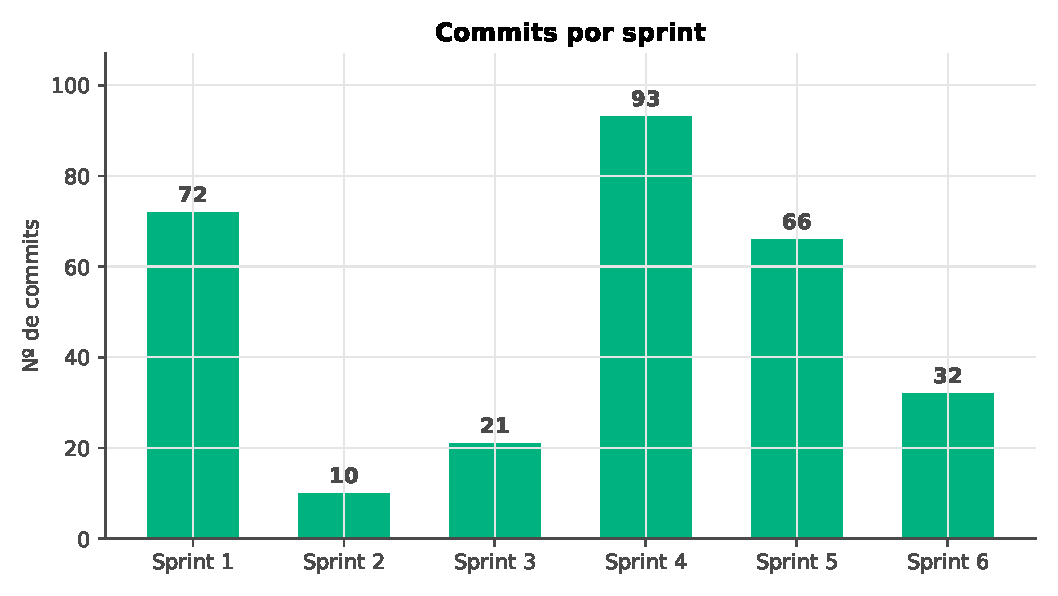
\includegraphics[width=0.85\textwidth]{figures/commits-per-sprint}
  \caption{Número de \emph{commits} reales por sprint en el repositorio Git.
  Refleja la actividad de desarrollo medida a partir del historial de
  \texttt{git log}; complementa los datos de esfuerzo estimado de la
  Tabla~\ref{tab:esfuerzo}.}
  \label{fig:commits-per-sprint}
\end{figure}

La Figura~\ref{fig:commits-per-sprint} muestra el reparto real de
\emph{commits} por sprint a partir del historial de Git, con la mayor
actividad concentrada en S1, S4 y S5 (en torno al 78\,\% del total).
La desviación global de +16,8\,\% se mantiene dentro del rango habitual
para proyectos individuales; el sprint con mayor desviación fue S5
(+37,5\,\%, problemas de integración del \emph{fingerprinting} con la
línea base) y el de menor desviación, S3 (+9,4\,\%, gracias a la
arquitectura de \emph{plugins} ya establecida en S2).

\subsection{Verificación del cumplimiento de objetivos}

El Cuadro~\ref{tab:cumplimiento} recoge, para cada objetivo específico, la
evidencia de su cumplimiento, el sprint en que se materializó y la subsección
donde se documenta.

\begin{table}[htbp]
  \centering
  \caption{Verificación del cumplimiento de los objetivos específicos}
  \label{tab:cumplimiento}
  \begin{tabularx}{\textwidth}{l X l c}
    \toprule
    \textbf{Obj.} & \textbf{Evidencia} & \textbf{Sprint} & \textbf{Estado} \\
    \midrule
    OE1 & Módulo de ingesta en formato \ac{CSV} con parseo robusto mediante
      matriz de \emph{fallback} (codificaciones $\times$ separadores);
      almacenamiento en MinIO; extracción automática de esquema;
      versionado padre-hijo con etiquetas personalizables.
      & S2 (sec.~\ref{sec:impl-ingesta}) & Cumplido \\
    OE2 & Siete métricas implementadas como \emph{plugins}; parametrización
      completa; sistema de pesos; plantillas reutilizables; ejecución
      asíncrona con Celery. & S3--S5 (sec.~\ref{sec:motor-metricas}) & Cumplido \\
    OE3 & Seis \emph{blueprints} funcionales planificados, ampliados a
      siete con la adición de \texttt{patterns} (validación
      reutilizable); autenticación \ac{JWT}; formato de respuesta
      estandarizado; paginación; validación Marshmallow.
      & S2 (sec.~\ref{sec:arq-backend}) & Superado \\
    OE4 & Más de 20 páginas; cuadros de mando interactivos; \ac{EDA} con
      histogramas, diagramas de caja y matrices de correlación; diseño
      adaptable. & S4 (sec.~\ref{sec:impl-frontend}) & Cumplido \\
    OE5 & Sistema de \emph{issues} con cuatro severidades;
      \emph{fingerprinting} \ac{SHA}-256; comparación con línea base;
      \emph{Quality Gates} con tres estados.
      & S5 (sec.~\ref{sec:impl-fingerprinting}) & Cumplido \\
    \bottomrule
  \end{tabularx}
\end{table}


Los cinco objetivos se cumplen con el sistema tal como está desplegado.  El
único objetivo superado es OE3: la \ac{API} creció de seis a siete
\emph{blueprints} funcionales durante el desarrollo, y los \emph{blueprints}
de organización técnica elevaron el total a diez.

\subsection{Cumplimiento de los requisitos no funcionales}
\label{sec:rnf-cumplimiento}

Más allá de los objetivos funcionales, el diseño de \dataqual ha prestado
atención a cinco requisitos no funcionales que han orientado sus decisiones
arquitectónicas y tecnológicas: \textbf{seguridad}, \textbf{escalabilidad},
\textbf{mantenibilidad}, \textbf{usabilidad} y \textbf{portabilidad}.  El
Cuadro~\ref{tab:rnf-cumplimiento} recoge, para cada uno, las decisiones de
diseño que lo materializan y su grado de cumplimiento (total o parcial).

\begin{table}[htbp]
  \centering
  \caption{Cumplimiento de los requisitos no funcionales}
  \label{tab:rnf-cumplimiento}
  \footnotesize
  \renewcommand{\arraystretch}{1.4}%
  \begin{tabularx}{\textwidth}{l X c}
    \toprule
    \textbf{RNF} & \textbf{Evidencia} & \textbf{Cumplimiento} \\
    \midrule
    Seguridad & Autenticación \ac{JWT} con \emph{tokens} de acceso y
      refresco; \emph{hashing} de contraseñas con \ac{PBKDF2}; limitación
      de tasa de peticiones (Flask-Limiter sobre Redis); validación de
      entradas con esquemas Marshmallow; lista de tokens prohibidos en
      las reglas de consistencia lógica para evitar la ejecución de
      código arbitrario; enmascaramiento automático de las columnas
      marcadas como \ac{PII} en todos los \emph{outputs}.  No se ha
      realizado una auditoría de seguridad ni pruebas de penetración
      formales. & Parcial \\
    Escalabilidad & Procesamiento asíncrono con Celery y Redis como
      \emph{broker}; arquitectura preparada para escalar
      horizontalmente el número de \emph{workers}; separación de
      responsabilidades entre los ocho servicios desplegados.  No se han
      realizado pruebas de carga con grandes volúmenes ni usuarios
      concurrentes. & Parcial \\
    Mantenibilidad & Arquitectura modular basada en \emph{blueprints},
      servicios y modelos; motor de métricas extensible mediante
      \emph{plugins} (\texttt{BaseMetric} + \texttt{METRIC\_REGISTRY});
      migraciones de base de datos versionadas con Alembic; separación
      estricta entre \emph{frontend} y \emph{backend}. & Total \\
    Usabilidad & Interfaz basada en Material Design con validación en
      tiempo real, notificaciones \emph{toast}, \emph{breadcrumbs} de
      navegación y estados de carga/error diferenciados; soporte
      español/inglés con cambio en tiempo real sin recargar la
      aplicación.  No se ha realizado una evaluación de usabilidad. & Parcial \\
    Portabilidad & Despliegue íntegro del \emph{stack} con un único
      \texttt{docker\,compose\,up}; configuración por variables de
      entorno; sin dependencias de servicios propietarios en la nube;
      ocho servicios orquestados conjuntamente. & Total \\
    \bottomrule
  \end{tabularx}
\end{table}

Quedan como verificación pendiente una \textbf{auditoría de seguridad}, la
\textbf{validación de escalabilidad mediante pruebas de carga} y una
\textbf{evaluación de usabilidad}, así como la \textbf{cobertura de pruebas
\emph{end-to-end} del \emph{frontend}}, que durante el desarrollo se validó
manualmente.  Estas tareas se recogen como trabajo futuro
(sección~\ref{sec:trabajo-futuro}).

%% =========================================================================
\section{Instanciación del marco \ac{ISO}/\ac{IEC} 5259 en DataQual}
\label{sec:instanciacion-iso5259}
%% =========================================================================

El marco normativo descrito en el capítulo~\ref{chap:antecedentes},
y en particular la taxonomía de
\ac{ISO}/\ac{IEC}~5259-2~\citep{iso5259} expuesta en la
sección~\ref{sec:alcance-metodologico}, permite estructurar las decisiones
de alcance de \dataqual en dos niveles.  El primero distingue qué
características son evaluables sobre el fichero de datos y cuáles requieren
acceso a infraestructura o metadatos externos, criterio derivado
directamente de la propia taxonomía.  El segundo nivel responde a
decisiones de priorización del propio proyecto: algunas características
técnicamente evaluables no fueron incluidas en esta versión por razones de
alcance, quedando como trabajo futuro.  La presente sección
detalla la instanciación resultante.

El Cuadro~\ref{tab:iso5259-cobertura} sintetiza la cobertura de \dataqual
respecto a las cuatro categorías de \ac{ISO}/\ac{IEC}~5259-2.

\begin{table}[htbp]
  \centering
  \caption{Cobertura de \dataqual respecto al modelo de calidad de \ac{ISO}/\ac{IEC} 5259-2}
  \label{tab:iso5259-cobertura}
  \footnotesize
  \renewcommand{\arraystretch}{2.0}%
  \begin{tabularx}{\textwidth}{l >{\raggedright\arraybackslash}p{5cm} l >{\raggedright\arraybackslash}X}
    \toprule
    \textbf{Categoría} & \textbf{Características} & \textbf{\dataqual} & \textbf{Motivo} \\
    \midrule
    Inherentes
      & Exactitud, Completitud, Consistencia, Actualidad
      & Implementadas
      & Extraíbles del dataset sin contexto externo \\
      & Credibilidad
      & Fuera de alcance
      & No priorizada en esta versión del proyecto; candidata para versiones futuras \\
    Mixtas
      & Accesibilidad, Conformidad, Eficiencia, Precisión, Trazabilidad, Confidencialidad, Comprensibilidad
      & Fuera de alcance
      & Requieren información del sistema que aloja el dato \\
    Dep.\ del sistema
      & Disponibilidad, Portabilidad, Recuperabilidad
      & Fuera de alcance
      & Determinadas por la infraestructura TI de la organización \\
    Adicionales (impl.)
      & Equilibrio (\texttt{class\_balance}), Diversidad (\texttt{diversity})
      & Implementadas
      & Impacto directo en fiabilidad y cumplimiento normativo de modelos de \ac{IA} \\
    Adicionales (técn.)
      & Efectividad, Relevancia, Representatividad, Similitud
      & Fuera de alcance
      & Requieren metadatos organizativos externos al fichero de datos \\
    Adicionales (futuro)
      & Identificabilidad, Auditabilidad, Puntualidad
      & Fuera de alcance
      & No priorizadas en esta versión del proyecto; candidatas para versiones futuras \\
    \bottomrule
  \end{tabularx}
\end{table}

\subsection{Características implementadas algorítmicamente}
\label{sec:caracteristicas-evaluables}

Las características inherentes de \ac{ISO}/\ac{IEC}~5259-2 (completitud,
exactitud sintáctica, consistencia y actualidad), junto con dos adicionales
(equilibrio de clases y diversidad), son evaluables algorítmicamente porque
sus métricas se calculan a partir de los propios valores del dataset, sin
acceder a sistemas externos ni conocer el dominio de negocio (el detalle de
cada cálculo se recoge en el Anexo~\ref{anx:metricas}).  Esta
\emph{auto-contención} es lo que ha hecho posible una herramienta que opera
exclusivamente sobre el fichero: el motor procesa cada \texttt{AnalysisRun}
de forma aislada, leyendo el dataset de MinIO y calculando las métricas sin
acceso a los sistemas de la organización propietaria.

\subsection{Características fuera del alcance}
\label{sec:caracteristicas-fuera-alcance}

Las características no incluidas (recogidas en el
Cuadro~\ref{tab:iso5259-cobertura}) responden a dos motivos.  La mayoría no
son evaluables sobre el fichero de datos de forma aislada, pues exigen acceso
a la infraestructura, a metadatos organizativos o al contexto de negocio del
que una herramienta externa no dispone: es el caso de las dependientes del
sistema (disponibilidad, portabilidad, recuperabilidad), las mixtas
(accesibilidad, conformidad, eficiencia, precisión, trazabilidad,
confidencialidad y comprensibilidad) y varias adicionales (representatividad,
relevancia, efectividad y similitud).  Otras, técnicamente abordables
(credibilidad, identificabilidad, auditabilidad y puntualidad), quedaron
fuera por priorización del proyecto y son candidatas para versiones futuras.

\subsection{Criterios de priorización aplicados}
\label{sec:priorizacion-mvp}

Entre las características algorítmicamente evaluables, el desarrollo de
\dataqual ha priorizado aquellas con mayor impacto en la fiabilidad de los
modelos de \ac{IA} y en el cumplimiento del marco normativo aplicable:

\begin{enumerate}
  \item \textbf{Las características inherentes de \ac{ISO}/\ac{IEC}~25012}
    (completitud, exactitud, consistencia y actualidad) implementadas a
    través de cinco métricas: \texttt{completeness},
    \texttt{syntactic\_accuracy}, \texttt{logical\_consistency},
    \texttt{currentness} y \texttt{uniqueness}, siendo esta última la
    sub-dimensión Con-ML-1 de consistencia definida en
    \ac{ISO}/\ac{IEC}~5259-2.  Esto proporciona cobertura directa de los
    requisitos de \ac{ISO}/\ac{IEC}~5259-2~\citep{iso5259} e
    \ac{ISO}/\ac{IEC}~25024~\citep{iso25024}.

  \item \textbf{Equilibrio de clases} (\texttt{class\_balance}), medido
    mediante la entropía de Shannon.  El desequilibrio de clases es uno de
    los factores documentados de sesgo en sistemas de
    \ac{IA}~\citep{amazon2018, buolamwini2018} y su corrección tiene un
    impacto directo en la equidad y fiabilidad de los modelos de
    clasificación.

  \item \textbf{Diversidad del dataset} (\texttt{diversity}): evalúa, de
    forma \emph{opt-in} con expectativas definidas por el usuario, si el
    dataset cubre los valores y rangos esperados por columna, detectando
    valores ausentes, categorías sub-representadas e intervalos numéricos
    sin datos, lo que puede comprometer la capacidad de generalización de
    los modelos entrenados con ese conjunto~\citep{iso5259}.
\end{enumerate}

Adicionalmente, los valores atípicos (\emph{outliers}) se han incorporado
como herramienta de diagnóstico en el módulo de \ac{EDA}, sin ser
computados como parte de la puntuación de calidad global.  Esta decisión
sigue explícitamente la recomendación de
\ac{ISO}/\ac{IEC}~5259-2~\citep{iso5259}, que no considera los \emph{outliers}
una dimensión de calidad inherente, sino un indicador diagnóstico cuya
relevancia depende del dominio de aplicación.

El resultado es una delimitación deliberada del alcance del proyecto:
\dataqual proporciona una evaluación algorítmica y estadística de las
características de calidad priorizadas para proyectos de \ac{IA}, aquellas
medibles directamente sobre el fichero de datos con mayor impacto en la
fiabilidad de los modelos.  Las características que requieren
infraestructura externa, metadatos organizativos o que no fueron
priorizadas en esta versión del proyecto quedan fuera de su ámbito actual,
configurándose como líneas de trabajo futuro.


% Local Variables:
%  coding: utf-8
%  mode: latex
%  mode: flyspell
%  ispell-local-dictionary: "castellano8"
% End:
